\documentclass[11pt]{article}

\usepackage[margin=1in]{geometry}
\usepackage{amsmath,amssymb}
\usepackage{booktabs}
\usepackage{array}
\usepackage{longtable}
\usepackage{graphicx}
\usepackage{hyperref}

\title{Materials Bridge Line B: Magnon Address Stability in alpha-Fe$_2$O$_3$ for HAOS-IIP}
\author{Tomislav Rupi\'c \\ Independent Researcher}
\date{May 2026}

\begin{document}

\maketitle

\begin{abstract}
This numbered update records release \texttt{65.1}: Materials Bridge Line B for HAOS-IIP. Line B is a bounded spin-sector materials bridge around coherent sub-THz magnon propagation in alpha-Fe$_2$O$_3$. It is a first-class repository artifact, but it is not yet a locally reproduced raw-data bridge. The current sidecar records a literature/user-audit-seeded persistence proxy of \texttt{0.902}, the reported group-velocity range \texttt{17.31--24.43 km/s}, micrometer-scale directional propagation, and the explicit raw-data boundary \texttt{NO\_PUBLIC\_STFT\_GRID\_FOUND}. The main literature anchor is Li et al., ``Anisotropic Coherent Propagation of Sub-Terahertz Magnons in Altermagnetic alpha-Fe$_2$O$_3$,'' DOI \href{https://doi.org/10.1002/adom.202503604}{\texttt{10.1002/adom.202503604}}. The secondary alpha-Fe$_2$O$_3$ control context is Yang et al., ``Spin-orbit torque manipulation of sub-terahertz magnons in antiferromagnetic alpha-Fe$_2$O$_3$,'' DOI \href{https://doi.org/10.1038/s41467-024-48431-w}{\texttt{10.1038/s41467-024-48431-w}}. This release does not claim a proof of HAOS-IIP, does not introduce a new magnon theory, and does not claim a \(k_\star\) result without raw sweep data. Its function is bookkeeping and boundary-setting: the alpha-Fe$_2$O$_3$ magnon address-stability prediction layer is now represented by an auditable sidecar artifact, while raw-data validation remains pending.
\end{abstract}

\tableofcontents

\section{Status and Scope}

This paper is release \texttt{65.1} in the HAOS-IIP numbered paper sequence.
It records:

\begin{itemize}
\item a new external spin-sector materials sidecar;
\item a first-class alpha-Fe$_2$O$_3$ magnon bridge artifact;
\item a bounded persistence summary seeded by a user-provided audit anchor and literature checks;
\item public-source references and explicit evidence class;
\item a raw-data boundary that prevents accidental overclaiming;
\item a link to the four magnon prediction records \texttt{HAOS-PRED-010} through \texttt{HAOS-PRED-013}.
\end{itemize}

The sidecar path is:

\begin{quote}
\path{experiments/materials_bridge/magnon_alpha_fe2o3_audit/}
\end{quote}

The release does not modify the HAOS-IIP frozen core, frozen phase artifacts,
telemetry definitions, theory files, prior experiments, or prior paper releases.

\section{Strict Non-Claims}

This release does not claim:

\begin{itemize}
\item that alpha-Fe$_2$O$_3$ proves HAOS-IIP;
\item that alpha-Fe$_2$O$_3$ embodies HAOS-IIP;
\item a new magnon theory;
\item a consciousness claim;
\item a raw-data external bridge pass;
\item a raw STFT/time-frequency recoverability result;
\item a \(k_\star\) detection or \(k_\star\) absence without raw sweep data.
\end{itemize}

The narrow question is:

\begin{quote}
Can the alpha-Fe$_2$O$_3$ magnon prediction layer be represented as a bounded
spin-sector materials bridge artifact while preserving the raw-data boundary?
\end{quote}

\section{Public Source Anchors}

The primary literature anchor is:

\begin{itemize}
\item Li et al., ``Anisotropic Coherent Propagation of Sub-Terahertz Magnons in Altermagnetic alpha-Fe$_2$O$_3$,'' \emph{Advanced Optical Materials}, 2026, DOI \href{https://doi.org/10.1002/adom.202503604}{\texttt{10.1002/adom.202503604}}.
\end{itemize}

The secondary alpha-Fe$_2$O$_3$ control context is:

\begin{itemize}
\item Yang et al., ``Spin-orbit torque manipulation of sub-terahertz magnons in antiferromagnetic alpha-Fe$_2$O$_3$,'' \emph{Nature Communications}, 2024, DOI \href{https://doi.org/10.1038/s41467-024-48431-w}{\texttt{10.1038/s41467-024-48431-w}}.
\end{itemize}

Line B uses these sources as literature anchors only. No source-data workbook,
CSV table, or full public time-frequency grid has been committed for local
reproduction in this release.

\section{Evidence Class}

\begin{center}
\begin{tabular}{p{0.30\linewidth}p{0.46\linewidth}}
\toprule
Field & Value \\
\midrule
Bridge line & \texttt{Materials Bridge Line B} \\
Material & \texttt{alpha-Fe2O3} \\
Status & literature/user-audit seeded pass \\
Data status & no raw public data loaded \\
Evidence class & literature report plus user-provided audit anchor \\
Raw STFT/time-frequency grid & no public validated grid found \\
Local reproduction & pending raw-data artifact \\
\bottomrule
\end{tabular}
\end{center}

This status is deliberately weaker than Line A's ferron bridge, where public
Figshare source files were downloaded, hashed, parsed, and audited locally.

\section{HAOS Translation}

The spin-sector readout maps into HAOS-style language as follows:

\begin{longtable}{p{0.27\linewidth}p{0.60\linewidth}}
\toprule
HAOS-facing term & Magnon-side read \\
\midrule
\endhead
carrier & antiferromagnetic / altermagnetic spin order \\
perturbation & crystal orientation, wavevector direction, thickness or boundary condition, magnetic field, pump delay \\
recoverable structure & coherent sub-THz exchange magnon packet \\
observable readout & time-resolved magneto-optical magnon traces, spectra, and propagation delay \\
visible failure & broadband thermalized response, amplitude collapse, loss of directional propagation, or no recoverable narrowband magnon feature \\
\bottomrule
\end{longtable}

This is a measurement dictionary. It does not assert a new ontology for magnons.

\section{Recorded Metrics}

\begin{center}
\begin{tabular}{p{0.34\linewidth}p{0.50\linewidth}}
\toprule
Metric & Value \\
\midrule
Persistence proxy & \texttt{0.902} \\
Persistence proxy status & user-provided, pending local reproduction \\
Reported group velocity minimum & \texttt{17.31 km/s} \\
Reported group velocity maximum & \texttt{24.43 km/s} \\
Reported group velocity span & \texttt{7.12 km/s} \\
Propagation status & micrometer-scale directional propagation reported in the literature \\
Spectral status & narrowband sub-THz exchange magnons reported in the literature \\
\(k_\star\) status & not claimed without raw sweep data \\
First visible failure status & not claimed without raw sweep data \\
\bottomrule
\end{tabular}
\end{center}

\begin{figure}[h]
\centering
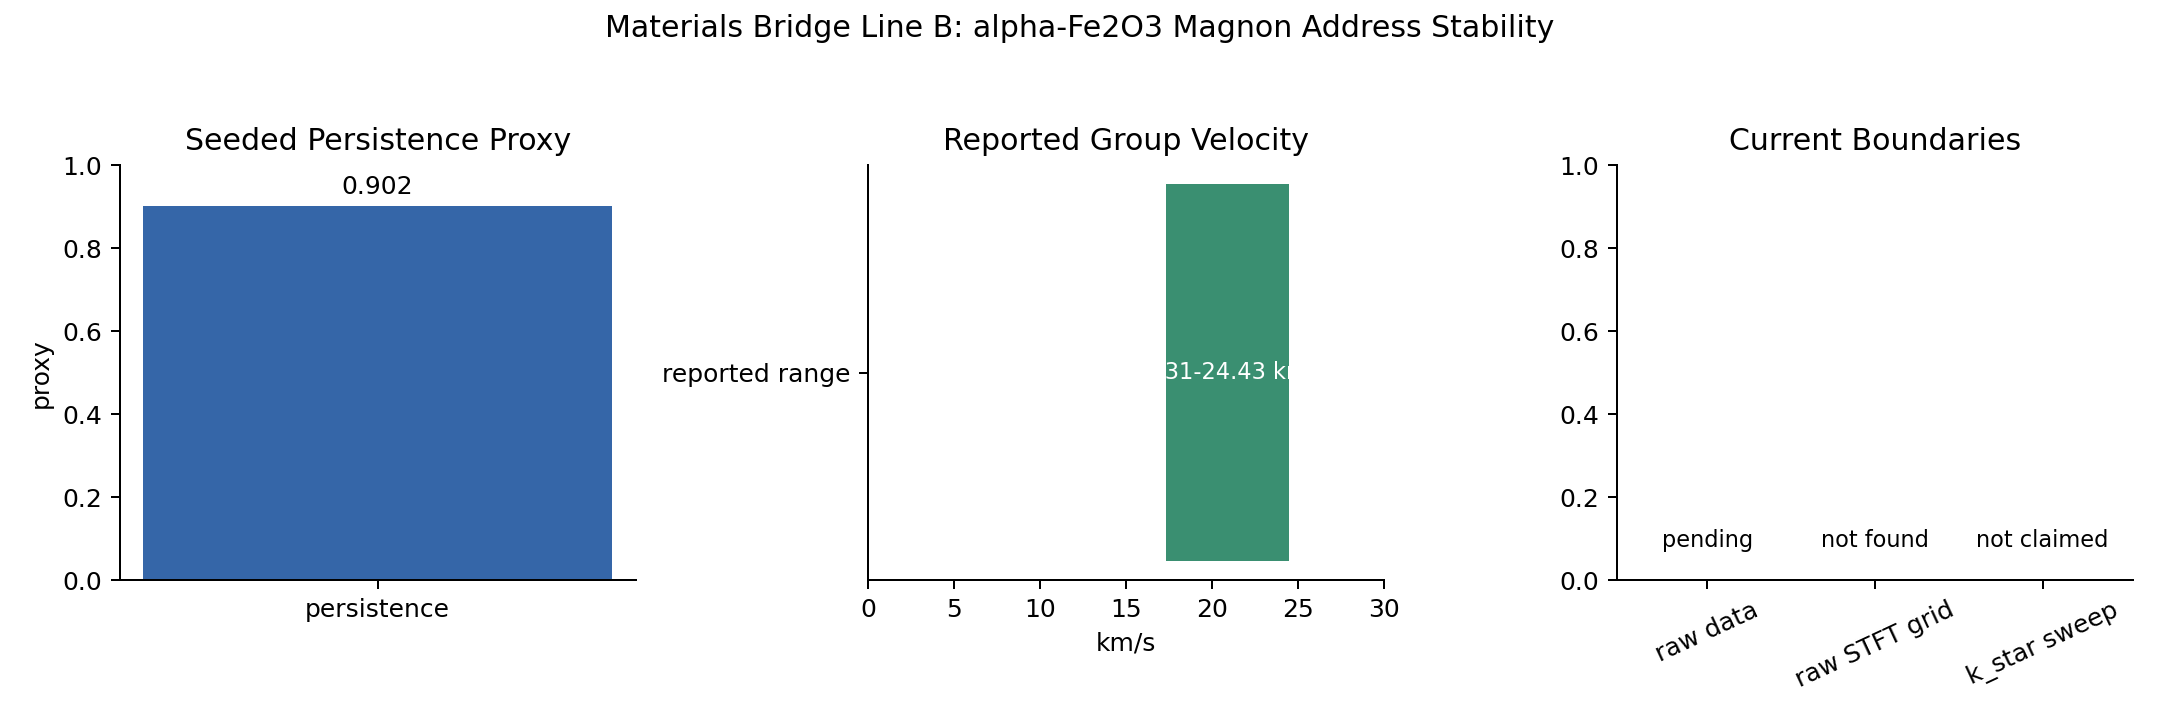
\includegraphics[width=0.92\linewidth]{../experiments/materials_bridge/magnon_alpha_fe2o3_audit/outputs/magnon_persistence_components.png}
\caption{Line B summary visualization. The persistence proxy is recorded as a seeded audit anchor; the group-velocity range is a literature-reported value; raw data, raw STFT grid, and \(k_\star\) sweep remain explicit boundaries.}
\end{figure}

\section{Relation to Prediction Ledger}

The magnon bridge supports four falsifiable prediction records:

\begin{longtable}{p{0.18\linewidth}p{0.70\linewidth}}
\toprule
Record & Short form \\
\midrule
\endhead
\texttt{HAOS-PRED-010} & crystal-orientation-dependent narrowband magnon address \\
\texttt{HAOS-PRED-011} & thickness / boundary dependent magnon group velocity \\
\texttt{HAOS-PRED-012} & magnon target-address recovery after perturbation \\
\texttt{HAOS-PRED-013} & hybrid magnon-phonon cross-sector locking \\
\bottomrule
\end{longtable}

Those records are prediction statements, not validation statements. Line B gives
them a dedicated sidecar anchor and states what must still be done before the
alpha-Fe$_2$O$_3$ case can be treated as a local raw-data bridge.

\section{Relation to Line A}

Line A and Line B are intentionally asymmetric:

\begin{longtable}{p{0.22\linewidth}p{0.33\linewidth}p{0.33\linewidth}}
\toprule
Field & Line A: ferron / NbOI$_2$ & Line B: magnon / alpha-Fe$_2$O$_3$ \\
\midrule
\endhead
Evidence class & real public data loaded and parsed & literature/user-audit seeded \\
Primary carrier & ferroelectric polarization order & antiferromagnetic / altermagnetic spin order \\
Primary readout & narrowband \(3.13\,\mathrm{THz}\) ferron feature and propagation traces & sub-THz coherent exchange magnons and directional propagation \\
Persistence proxy & \texttt{0.957192} & \texttt{0.902} \\
Raw STFT grid & \texttt{NO\_STFT\_DATA\_FOUND} for Figshare XLSX grid & \texttt{NO\_PUBLIC\_STFT\_GRID\_FOUND} \\
Raw-data status & \texttt{REAL\_DATA\_LOADED} & \texttt{NO\_RAW\_PUBLIC\_DATA\_LOADED} \\
\(k_\star\) & no collapse detected under current proxy thresholds & not claimed without raw sweep \\
\bottomrule
\end{longtable}

This distinction matters. Line A is a real-data bridge. Line B is a structured
spin-sector bridge artifact awaiting raw-data reproduction.

\section{Required Next Work}

Line B becomes a stronger external-data bridge only if a future sidecar can:

\begin{itemize}
\item locate public alpha-Fe$_2$O$_3$ time-domain or spectral data tables;
\item record provenance, URLs, timestamps, and SHA256 hashes;
\item parse time traces, spectra, or time-frequency grids without digitizing plots;
\item compute recoverability, propagation delay, group velocity, and spectral stability locally;
\item run deterministic \(k_\star\), safety-margin, confidence, and visible-failure logic;
\item preserve a clean \texttt{NO\_PUBLIC\_STFT\_GRID\_FOUND} status if no raw grid exists.
\end{itemize}

Until that happens, the correct status remains:

\begin{quote}
\texttt{PASS\_LITERATURE\_USER\_AUDIT\_SEEDED}, not \texttt{REAL\_DATA\_LOADED}.
\end{quote}

\section{Conclusion}

Materials Bridge Line B makes the alpha-Fe$_2$O$_3$ magnon address-stability
layer explicit, numbered, and auditable. It records the current seeded
persistence proxy \texttt{0.902}, the reported velocity range
\texttt{17.31--24.43 km/s}, and the public raw-grid boundary
\texttt{NO\_PUBLIC\_STFT\_GRID\_FOUND}. The safe claim is narrow: the spin-sector
prediction layer is now represented by a bounded sidecar artifact, and the repo
plainly distinguishes it from the real-data ferron bridge.

\end{document}
